\section{EK-KOR2 Execution Layer}
\label{sec:ekkor2}

The \ekkor{} system provides the real-time execution layer that implements planned paths through distributed coordination. This section describes the architecture, potential field scheduling, topological coordination, and consensus protocols.

\subsection{System Architecture}

\ekkor{} implements a two-tier architecture separating application-layer coordination (L1) from safety-critical supervision (L2).

\textbf{L1 Application Layer:} Executes on STM32G474 microcontrollers at 170 MHz. Each module runs:
\begin{itemize}
    \item Individual power electronics control (PFC, DC-DC conversion)
    \item ROJ (swarm) intelligence coordination algorithms
    \item Distributed load balancing through potential fields
    \item Fleet-level optimization via emergent behavior
\end{itemize}

\textbf{L2 Safety Layer:} Executes on AURIX TC375 with ASIL-D certification, providing:
\begin{itemize}
    \item Grid protection (frequency, voltage monitoring)
    \item Emergency shutdown authority
    \item Independent health monitoring
    \item Compliance logging
\end{itemize}

The network employs hierarchical CAN-FD segments: 10-20 segments of 50-100 modules each, connected through gateways to a backbone monitored by L2.

\begin{figure}[htbp]
\centering
% System Architecture: Planning → Execution data flow
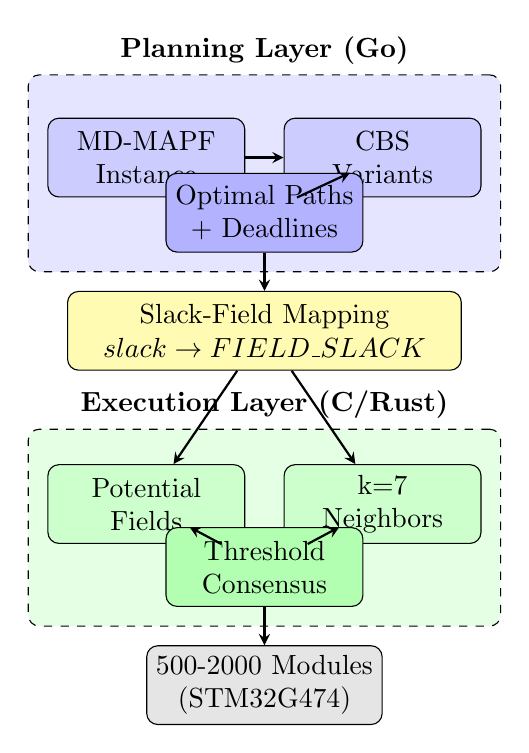
\begin{tikzpicture}[
    box/.style={draw, rounded corners, minimum width=2.5cm, minimum height=1cm, align=center},
    bigbox/.style={draw, rounded corners, minimum width=6cm, minimum height=2.5cm, align=center, dashed},
    arrow/.style={->, >=stealth, thick}
]

% Planning Layer
\node[bigbox, fill=blue!10] (planning) at (0, 3) {};
\node[above] at (planning.north) {\textbf{Planning Layer (Go)}};

\node[box, fill=blue!20] (mdmapf) at (-1.5, 3.2) {MD-MAPF\\Instance};
\node[box, fill=blue!20] (cbs) at (1.5, 3.2) {CBS\\Variants};
\node[box, fill=blue!30] (paths) at (0, 2.5) {Optimal Paths\\+ Deadlines};

\draw[arrow] (mdmapf) -- (cbs);
\draw[arrow] (cbs) -- (paths);

% Bridge
\node[box, fill=yellow!30, minimum width=5cm] (bridge) at (0, 1) {Slack-Field Mapping\\$\text{slack} \rightarrow \text{FIELD\_SLACK}$};

\draw[arrow] (paths) -- (bridge);

% Execution Layer
\node[bigbox, fill=green!10] (execution) at (0, -1.5) {};
\node[above] at (execution.north) {\textbf{Execution Layer (C/Rust)}};

\node[box, fill=green!20] (field) at (-1.5, -1.2) {Potential\\Fields};
\node[box, fill=green!20] (k7) at (1.5, -1.2) {k=7\\Neighbors};
\node[box, fill=green!30] (consensus) at (0, -2) {Threshold\\Consensus};

\draw[arrow] (bridge) -- (field);
\draw[arrow] (bridge) -- (k7);
\draw[arrow] (field) -- (consensus);
\draw[arrow] (k7) -- (consensus);

% Hardware
\node[box, fill=gray!20] (hw) at (0, -3.5) {500-2000 Modules\\(STM32G474)};
\draw[arrow] (consensus) -- (hw);

\end{tikzpicture}

\caption{System architecture showing data flow from MD-MAPF planning through slack-field mapping to distributed execution on embedded modules.}
\label{fig:architecture}
\end{figure}

\subsection{Potential Field Scheduler}

The potential field scheduler replaces priority-based scheduling with gradient-mediated coordination, adapting Khatib's~\cite{khatib1986potential} formulation to the temporal scheduling domain.

\begin{definition}[Coordination Field]
Each module maintains a coordination field structure:
\begin{equation}
F = (\Phi_{\text{load}}, \Phi_{\text{thermal}}, \Phi_{\text{power}}, \Phi_{\text{slack}}, t_{\text{stamp}}, \text{seq})
\end{equation}
published to neighbors via CAN-FD every 50ms.
\end{definition}

\textbf{Load Potential:} Exponential decay with $\tau = 100$ms:
\begin{equation}
\Phi_{\text{load}}(t) = \Phi_{\text{load}}(t_0) \cdot e^{-(t-t_0)/\tau}
\end{equation}

\textbf{Deadline Attraction:} Inverse slack creates urgency:
\begin{equation}
U_{\text{deadline}} = k_d \cdot (\text{slack})^{-1}, \quad F_{\text{deadline}} = k_d / \text{slack}^2
\end{equation}

\textbf{Resource Repulsion:} Prevents contention:
\begin{equation}
U_{\text{rep}} = k_r \cdot e^{-\alpha \cdot d_{ij}}
\end{equation}
where $d_{ij}$ measures contention proximity.

Implementation uses Q15 fixed-point format (1.15 representation, range $[-1, +1)$) for gradient storage, with Q31 intermediate products to prevent overflow. Lock-free double-buffering with sequence counters ensures consistency without blocking.

\subsection{Topological k=7 Coordination}

The breakthrough insight from Cavagna and Giardina's study of starling flocks~\cite{cavagna2010scale} reveals that scale-free correlations emerge when individuals interact with a fixed number of \emph{topological} neighbors regardless of distance.

\begin{definition}[Topological Neighbor Set]
Each module maintains exactly $k=7$ logical neighbors:
\begin{equation}
\mathcal{N}_k(i) = \{j_1, \ldots, j_7\} \quad \text{where} \quad |\mathcal{N}_k(i)| = 7
\end{equation}
selected by logical distance metric independent of physical CAN topology.
\end{definition}

\textbf{Key Properties:}
\begin{itemize}
    \item \textbf{Scale-Free Correlation:} Information propagates without attenuation; correlation length scales linearly with network size
    \item \textbf{Bandwidth Efficiency:} Each node exchanges data with 7 neighbors, not all $N-1$ peers, reducing traffic by factor $\approx N/7$
    \item \textbf{Fault Tolerance:} With $k=7$, the system tolerates up to 2 Byzantine faults per node while achieving consensus (satisfies $N \geq 3f + 1$)
\end{itemize}

\begin{algorithm}
\caption{Neighbor State Update}
\label{alg:neighbor}
\begin{algorithmic}[1]
\REQUIRE Heartbeat from sender\_id with load value
\IF{sender\_id $\in \mathcal{N}_k$}
    \STATE Update neighbor\_load[sender\_id]
    \STATE Reset missed\_heartbeats[sender\_id] $\leftarrow 0$
    \STATE neighbor\_state[sender\_id] $\leftarrow$ \textsc{Healthy}
\ENDIF
\end{algorithmic}
\end{algorithm}

Fault detection triggers when a neighbor misses 3 consecutive heartbeats, initiating Byzantine-tolerant consensus among remaining neighbors.

\begin{figure}[htbp]
\centering
% k=7 Topology: Scale-free neighbor network
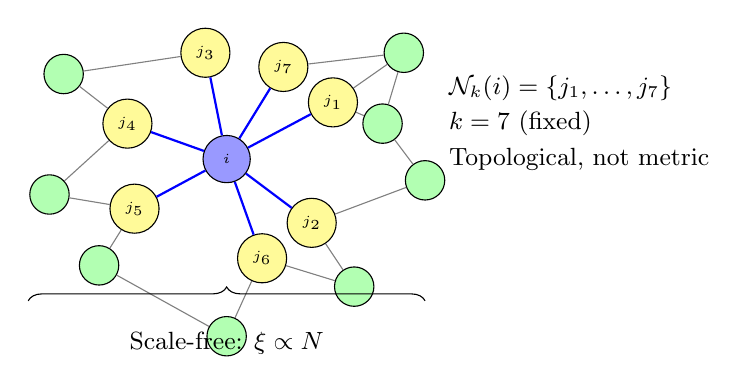
\begin{tikzpicture}[
    scale=0.9,
    node/.style={circle, draw, fill=green!30, minimum size=0.5cm, font=\tiny},
    central/.style={circle, draw, fill=blue!40, minimum size=0.6cm, font=\tiny},
    neighbor/.style={circle, draw, fill=yellow!40, minimum size=0.5cm, font=\tiny},
    edge/.style={draw, gray},
    highlight/.style={draw, blue, thick}
]

% Central node
\node[central] (c) at (0, 0) {$i$};

% k=7 neighbors (highlighted)
\node[neighbor] (n1) at (1.5, 0.8) {$j_1$};
\node[neighbor] (n2) at (1.2, -0.9) {$j_2$};
\node[neighbor] (n3) at (-0.3, 1.5) {$j_3$};
\node[neighbor] (n4) at (-1.4, 0.5) {$j_4$};
\node[neighbor] (n5) at (-1.3, -0.7) {$j_5$};
\node[neighbor] (n6) at (0.5, -1.4) {$j_6$};
\node[neighbor] (n7) at (0.8, 1.3) {$j_7$};

% Other nodes (not neighbors)
\node[node] (o1) at (2.5, 1.5) {};
\node[node] (o2) at (2.8, -0.3) {};
\node[node] (o3) at (-2.3, 1.2) {};
\node[node] (o4) at (-2.5, -0.5) {};
\node[node] (o5) at (0, -2.5) {};
\node[node] (o6) at (1.8, -1.8) {};
\node[node] (o7) at (-1.8, -1.5) {};
\node[node] (o8) at (2.2, 0.5) {};

% Highlighted edges (k=7 neighbors)
\draw[highlight] (c) -- (n1);
\draw[highlight] (c) -- (n2);
\draw[highlight] (c) -- (n3);
\draw[highlight] (c) -- (n4);
\draw[highlight] (c) -- (n5);
\draw[highlight] (c) -- (n6);
\draw[highlight] (c) -- (n7);

% Other edges (network connections)
\draw[edge] (n1) -- (o1);
\draw[edge] (n1) -- (o8);
\draw[edge] (n2) -- (o2);
\draw[edge] (n2) -- (o6);
\draw[edge] (n3) -- (o3);
\draw[edge] (n4) -- (o3);
\draw[edge] (n4) -- (o4);
\draw[edge] (n5) -- (o4);
\draw[edge] (n5) -- (o7);
\draw[edge] (n6) -- (o5);
\draw[edge] (n6) -- (o6);
\draw[edge] (n7) -- (o1);
\draw[edge] (o1) -- (o8);
\draw[edge] (o2) -- (o8);
\draw[edge] (o5) -- (o7);

% Legend
\node[right, font=\small] at (3, 1) {$\mathcal{N}_k(i) = \{j_1, \ldots, j_7\}$};
\node[right, font=\small] at (3, 0.5) {$k = 7$ (fixed)};
\node[right, font=\small] at (3, 0) {Topological, not metric};

% Annotation
\draw[decorate, decoration={brace, amplitude=5pt}] (-2.8, -2) -- (2.8, -2);
\node[below, font=\small] at (0, -2.3) {Scale-free: $\xi \propto N$};

\end{tikzpicture}

\caption{Topological $k=7$ neighbor coordination. Each node maintains exactly 7 logical neighbors regardless of physical distance, enabling scale-free correlation propagation.}
\label{fig:k7}
\end{figure}

\subsection{Threshold Consensus Protocol}

Distributed decision-making for system-wide transitions uses threshold consensus inspired by quorum sensing in biological systems.

\begin{definition}[Consensus Thresholds]
Decision categories require different agreement levels:
\begin{itemize}
    \item \textbf{Safety-critical} (emergency stop, grid disconnect): 67\% supermajority
    \item \textbf{Operational} (power ramping, load redistribution): 50\% majority
    \item \textbf{Local} (thermal throttling): Autonomous, no consensus
\end{itemize}
\end{definition}

\begin{definition}[Consensus Vote]
A vote structure contains:
\begin{equation}
v = (\text{proposal\_id}, \text{weight}, \text{inhibit\_mask}, \text{MAC})
\end{equation}
where weight reflects module health score and inhibit\_mask suppresses competing proposals.
\end{definition}

\textbf{Mutual Inhibition:} When voting for proposal $A$, inhibition bits are set for incompatible proposals (e.g., both ``increase power'' and ``decrease power''). The consensus calculation excludes inhibited votes.

\textbf{Density-Dependent Activation:} Thresholds adjust based on participating module count, preventing small subsets from achieving consensus on fleet-wide decisions.

\subsection{Network Partition Handling}

Network partitions require detection, split-brain prevention, and graceful recovery.

\textbf{Detection:} Three complementary mechanisms:
\begin{enumerate}
    \item Heartbeat-based suspicion (3 missed heartbeats)
    \item Quorum monitoring (visible nodes $< N/2 + 1$)
    \item CAN arbitration analysis (missing high-priority IDs)
\end{enumerate}

\textbf{Split-Brain Prevention:} Only the majority partition continues consensus decisions. The minority partition enters freeze mode:
\begin{itemize}
    \item Local droop-only power control
    \item Suspended leader election and voting
    \item Maintained last-known setpoints
    \item Continued local safety functions
\end{itemize}

\textbf{Epoch-Based Reconciliation:} Each partition event increments a global epoch counter. When connectivity restores, a three-phase protocol executes:
\begin{enumerate}
    \item \textbf{Leader Resolution:} Highest epoch leader continues
    \item \textbf{State Synchronization:} Minority requests deltas from majority
    \item \textbf{Load Reintegration:} 10-second ramp with 100ms steps
\end{enumerate}

\subsection{Planning-Execution Bridge}

The MAPF-HET planning layer interfaces with \ekkor{} through two mechanisms:

\textbf{1. Slack Field Component:}
\begin{equation}
\text{EKK\_FIELD\_SLACK} = \text{clamp}\left(\frac{\text{slack\_us}}{\tau_{\text{norm}}}, 0, 1\right)
\end{equation}
Published as the 6th field component, enabling deadline-aware gradient coordination.

\textbf{2. Capability Bitmask:}
\begin{equation}
\text{can\_perform}(\text{have}, \text{need}) = (\text{have} \land \text{need}) = \text{need}
\end{equation}
Enables heterogeneous task assignment based on module capabilities (thermal status, V2G support, gateway role).

The gradient mechanism naturally prioritizes tight-deadline modules:
\begin{equation}
\nabla\Phi_{\text{slack}} < -\theta \Rightarrow \text{offer assistance to neighbors}
\end{equation}

This creates emergent load balancing where resources flow toward deadline-constrained modules without central coordination.
